%!TEX root = /Users/rafaeldurelli/Dropbox/Artigos Elaborados/KDM propagation_2015/sbes_2015_kdm_propagation/sbes2015_kdm_propagation.tex

\section{Propagation-Aware Refactorings} % (fold)
\label{sec:the_approach}

In order to fulfill the limitation pointed out, we introduce an approach that aims to propagate all the changes throughout the KDM's levels. This approach ensures that when a change/refactoring is performed in any KDM's level, it is correctly propagated to the affected KDM's levels and vice versa. So it make certain that the consistency between the KDM's levels when they are refactored. 
The described problem presented in Section~\ref{sec:motivation_and_running_example} can, in our view, be split into three steps, which are depicted by its corresponding letters and tittle in Figure~\ref{fig:approach}. 

%According to the literature, there are two possibilities to perform propagation in models (colocar ref). One possibility is to mark the modifications on the source KDM's model without actually commiting them until the end of the transformation, so that expression evaluation can occur on the original source KDM's model by ignoring the modifications. Another possibility is to first compute the set of basic operations to perform, storing this set in an external artifact representation and then apply all the changes at once. Our approach follows the second possibility and it is divided in three steps, which are depicted by its corresponding letters and tittle in Figure~\ref{fig:approach}.


\begin{figure}[h]
	\centering
	% Requires \usepackage{graphicx}
	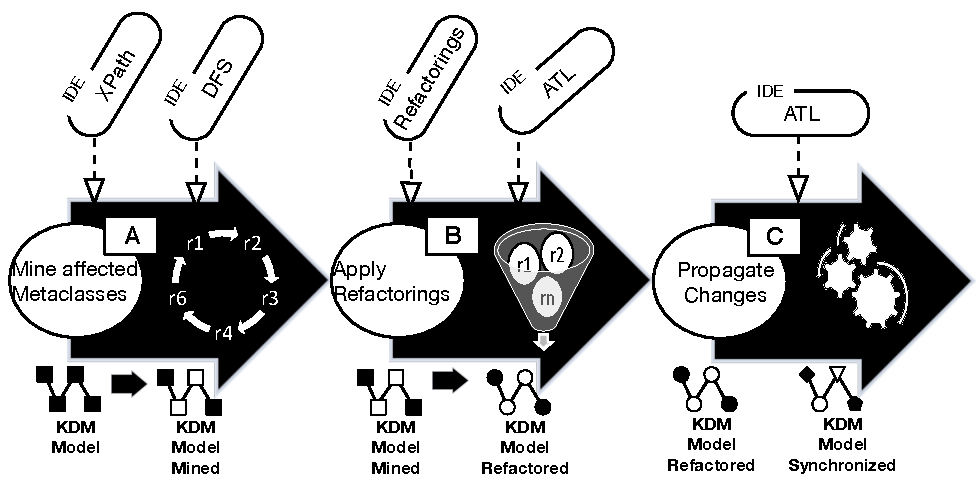
\includegraphics[scale=0.56]{figuras/allStepApproachKDMPropagation}
	\caption{Propagation-Aware Refactorings steps.}
	\label{fig:approach}
\end{figure}

In the step [A], \textit{Mine Affected Metaclasses}, we developed a mechanism which shows all metaclasses that need to be updated after applying any changes/refactoring. These metaclasses are those that have some dependence on the metaclass to be modified by the refactoring. This step is totally based on a set of queries that works on a KDM instance. In fact, this step uses depth-first search algorithm to identify all affected metaclasses along with a set of queries.

In step [B], \textit{Apply Refactoring}, here the software modernizer has to choose an appropriate refactoring to be applied into the KDM. In this step, new metaclasses can be created, updated, and removed. Also it is necessary to gather all the needed parameters for applying the refactoring. %that the software modernizer inputs all the needs parameters for applying the refactoring is gathered.  %The most frequent modification to the KDM instances in this scenario will be, intuitively, creating new metaclasses. However, updating existing metaclasses with their relationship will be frequent as well. In simpler cases, updating means changing properties of existing metaclasses. In more complex cases, updating means removing metaclasses and replacing them with new and refactored ones.
This step uses M2M transformation language to perform the refactorings.

In step [C], \textit{Propagate Changes}, involves updating the elements identified in the step [A].  As in step [B], in this step we also have used M2M to update all KDM's instances. 
More details on each step are provided in the next sections.

\subsection{Mine Affected Metaclasses} % (fold)
\label{sub:mine_affected_metaclasses}

The step [A] starts with a depth-first search algorithm that aims to show all metaclasses and its relationships that use somehow the metaclass(es) that will be refactored in step [B]. As input all the metaclasses that will be used to apply an specific refactoring is needed. The algorithm uses a set of queries. These queries are performed on the KDM's instance to mine all the affected/linked metaclasses. All the queries were created using XPath. We have decided to use XPath because it is a well-know and well-documented language. 

Let us consider the running example depicted in Figure~\ref{fig:system}. In this example, the engineer aims to apply the refactoring \textit{Move Class} - both classes \texttt{Student} and \texttt{Instructor} should not longer be contained in the package \texttt{View}. These classes should be allocated into the package \texttt{Model}. Considering the refactoring \textit{Move Class}, three elements (\texttt{Student}, \texttt{Instructor}, and their package) need to be investigated throughout the KDM's instance in order to identify propagation scenarios of changes. 

Therefore, firstly a query must be executed to get the root elements in KDM. This query is represented as the first statement in Figure~\ref{fig:queriesXPath}, see line 1 - it is used to return an instance of the metaclass \texttt{Segment}. The returned Segment, as well as all KDM's levels are gathered by the other queries presented in Figure~\ref{fig:queriesXPath} lines 2 to 5. The returned elements of these queries are used as input in our depth-first search algorithm.

\begin{figure}[h]
	\centering
	% Requires \usepackage{graphicx}
	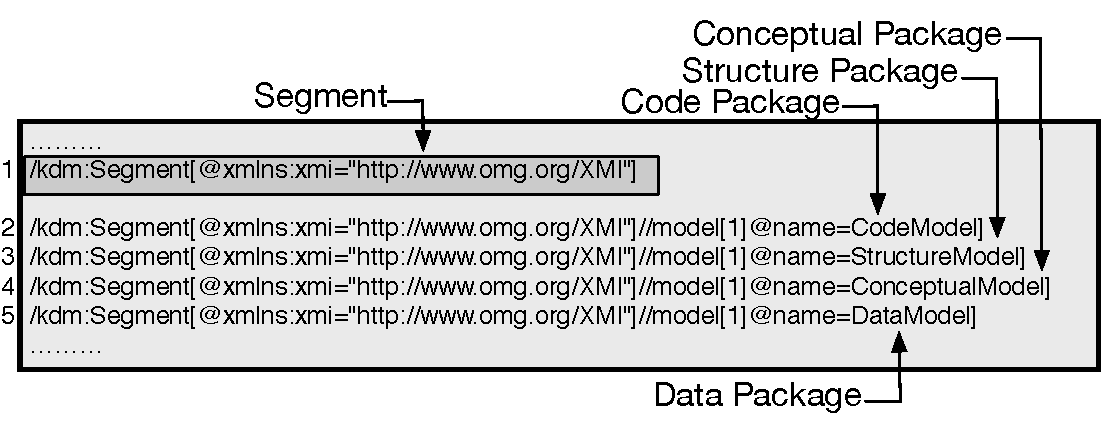
\includegraphics[scale=0.479]{figuras/queiresANDATLSBESNew}
	\caption{Xpath used to return the KDM's root element, Segment.}
	\label{fig:queriesXPath}
\end{figure}


\begin{algorithm}[h]
     \SetAlgoLined
     \KwIn{DFS (G, u, eL) where G is a KDM's instance, u is the initial metaclass, i.e., Segment, and eL is a set of elements to verify}
     \KwOut{A collection of affected metaclasses}
     \Begin{
     \ForEach{$outgoing$ edge e = (u, v) of u} {
	\If{vertex v as has not been visited }{
			\If{vertex v contain implementation = true }{
				
				\ForEach{$implementations$ element}{
				verify all elements in implementation
				}
				Mark vertex v as visited (via edge e).
				Recursively call DFS (G, v).
			}
			
				}				
			}		
	
	}
     \caption{DFS(G,u) - Depth-First Search Algorithm.}
     \label{alg:death1}
   \end{algorithm}

Algorithm~\ref{alg:death1} depicts the depth-first search algorithm that is used to mine all the affected metaclasses. It takes as input a KDM's instance, a \texttt{Segment}, and a set of elements that will be refactored in Step [B] (e.g., for the refactoring \textit{Move Class} three affected elements - \texttt{Student}, \texttt{Instructor}, and their package) depicted in Figure~\ref{fig:queriesXPath}. A diagram of how our depth-first search algorithm works is shown in Figure~\ref{fig:algWorks2}. Each node represents a metaclass and the edges represent the relationship among the metaclasses - the node A represents the \texttt{Segment} and K, H, E and B illustrate \texttt{CodeModel}, \texttt{StructureModel}, \texttt{ConceptualModel}, and \texttt{DataModel}, respectively. 

More specifically, the algorithm works as follows: first it is necessary to pick a starting point, i.e., the metaclass \texttt{Segment}. Visit the \texttt{Segment}, push it onto a stack, and mark it as visited. Then it is necessary to go to the next metaclass that is unvisited, verify if it has an association named \texttt{implementation}. If yes, it verifies if this association contains references to any element's used in the refactoring, if yes - push it on the stack, and mark it. This continues until the algorithm reachs the last metaclass. Then the algorithm checks to see if the \texttt{Segment} has any unvisited adjacent metaclass. If it does not, then it is necessary to pop it off the stack and check the next metaclass. If the algorithm finds one (unvisited metaclass), it starts visiting adjacent metaclasses until there are no more, check for more unvisited adjacent metaclasses, and continue the process always verifying the association named implementation. When the algorithm finally reach the last metaclass on the stack and there are no more adjacent, unvisited metaclasses that contains the association \texttt{implementation} without check , our algorithm should show a list of all affected metaclasses. 
%
%
%
%
%
%
%
%
%

\begin{figure}
	\centering
	% Requires \usepackage{graphicx}
	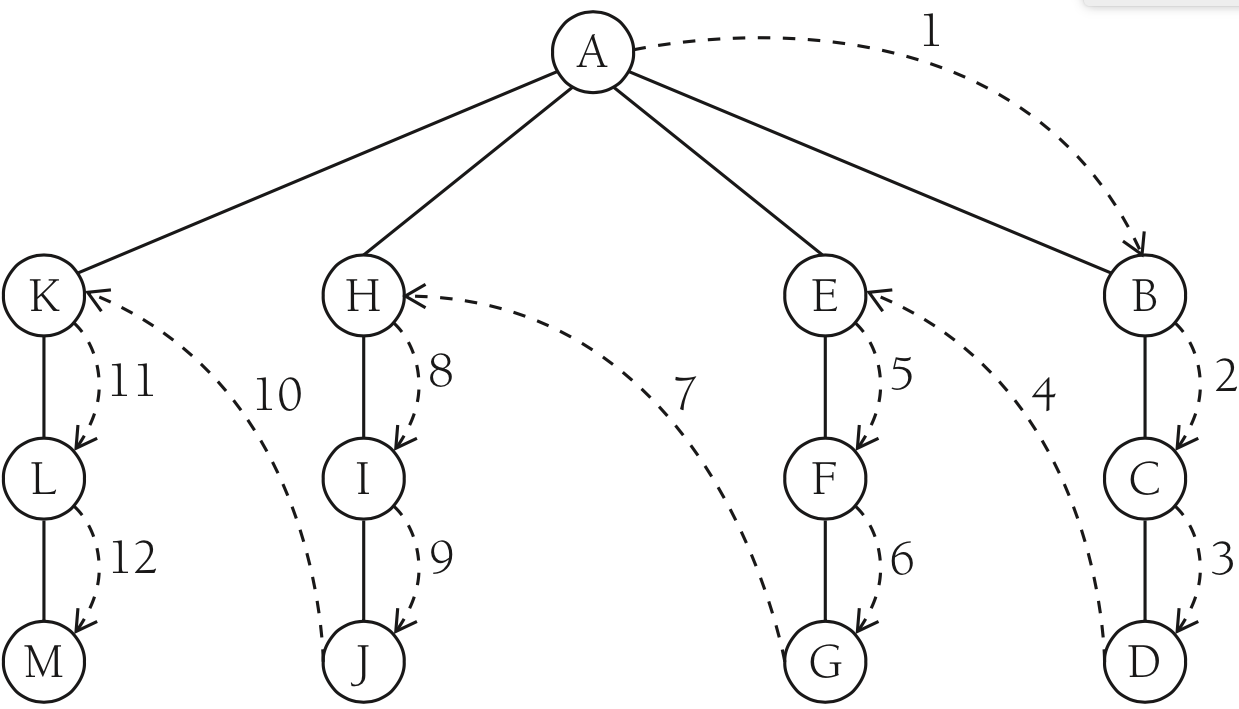
\includegraphics[scale=0.2]{figuras/algWorks2}
	\caption{Depth-First Search.}
	\label{fig:algWorks2}
\end{figure}






%As can be visualized, a stack is used to store all affected elements, see Algorithm~\ref{alg:death1} line 2, \ding{182}. In line 3 a generic KDM element is defined. While \textit{seg} is non-empty, a node is chosen for expansion (line 4). %For fact edges, the dependency of the edge on the particular fact that caused its creation is then recorded (lines 14- 16)





%\begin{algorithm}[h]
%     \SetAlgoLined
%     \KwIn{KDMEntity kdmElement, Segment segment, KDMModel model}
%     \KwOut{All affected metaclasses}
%     \Begin{
%   $ Stack stack \longleftarrow \{\}$\;
%   KDMEntity elementToVerify\;
%     \ForEach{$seg$ in $segment$} {
%	\eIf{seg.getOwnedElements() != null}{
%			\If{seg.getNextSiblind() != null}{
%				$elementToVerify \longleftarrow seg.getNextSiblind()$\;
%		\If{\ding{182} isAffected(elementToVerify, kdmElement, model)}{
%					stack.push(elementToVerify)\;
%					$seg \longleftarrow  seg.getFirstChild()$\;
%				}				
%			}		
%	
%	}{ $seg \longleftarrow seg.getNextSiblind()$\;
%		\If{seg = null \&\& stack.isEmpty()}{
%			// return to the parent's level
%		}
%	}
%     }
%	\ding{184} \Return{stack}
%     }
%     \caption{Depth-First Search Algorithm.}
%     \label{alg:death1}
%   \end{algorithm}
%
%\begin{algorithm}[h]
%     \SetAlgoLined
%     \KwIn{KDMEntity kdmElement, KDMModel model, KDMEntity e}
%     \KwOut{true or false}
%     \Begin{
%     	\If{ (e = AbstractUIElement) or (e = AbstractStructureElement) or (e = BuildResource) or (e = AbstractPlatformElement) or (e = AbstractConceptualElement) or (e = AbstractEventElement)
%				} {
%					     \ForEach{$elements$ in $e.getImplementation()$} {
%					\If{ elements = ele} {
%					\Return{true}
%					}
%					}				
%				}
%\uElseIf{ e = AbstractDataElement
%				} {
%					     \ForEach{$elements$ in $elementToV.getDataRelation()$} {
%					\If{ elements = elementToVerify} {
%					\Return{true}
%					}
%					}				
%				}
%	...
%     }
%     \caption{isAffected Algorithm}
%     \label{alg:death}
%   \end{algorithm}

%As every element, except the Segment, is connected somehow it is necessary to iterate throughout them, line 4 of Algorithm~\ref{alg:death} illustrates this iteration. After, the method \texttt{isAffected(...)} is called to verify if the element is affected.  If the condition in line 8 evaluates to true, then the element is pushed into the stack defined in line 2. Finally, in line 20 the stack is returned with all affected elements, see Algorithm~\ref{alg:death} \ding{184}. 

\subsection{Apply Refactoring} % (fold)
\label{sub:apply_refactoring}

In the step [B] the engineer must apply the refactoring. A natural way of implementing refactoring in models is by means of \textit{in-place transformations}\footnote{We have devised a repository where a set of \textit{in-place transformations} (i.e., refactoring) is available. The repository can be accessed in www.site.com.br. It aims is to share refactoring to be applied into KDM's instances.} as describe in Section~\ref{sec:background}. %This kind of transformations are used for rewriting a model by creating, deleting, and updating elements in the input model, e.g., in a KDM's instance. 
Going into more details, applying these transformations/refactoring into a KDM's instance can introduce incompatibilities and inconsistencies which can not be easily resolved. In fact, we can classified these transformations by their corrupting or non-corrupting effects:%\cite{towardssynchronizing07}:

\begin{itemize}
\item \textit{non-breaking changes}: changes which do not break the KDM's instance - for instance, the refactoring rename;

\item \textit{breaking and resolvable changes automatically}: changes which do break the KDM instance, but can be resolved by automatic means - for instance, apply the refactoring \textit{move class, extract class, push meta-attributes}, etc;

\item \textit{breaking and unresolvable changes automatically}: changes which do break the KDM instance and can not be resolved automatically - for instance, when manual interventions are needed.
%
\end{itemize} 
% In the context of this paper, we are only considering the \textit{non-breaking changes} and \textit{breaking and resolvable changes automatically}. 
%
These transformations can be performed by means of rule-based languages. Our approach uses ATL Transformation Language (ATL). The main advantage of using one ATL is that the transformation logic can be expressed at a high level of abstraction thus enhancing maintainability and understandability. 

To express a transformation in our approach, the user must specify mapping rules that describe how KDM's elements model can be refactored. Further, the users should inform some input parameters that should be properly instantiated. For example, considering the refactoring \textit{Move Class}, an ATL transformation that could perform this task is depicted in Figure~\ref{fig:ATLRefactoring}.








%A natural way of implementing refactoring in models is by means of \textit{in-place transformations}\footnote{The term \textit{in-place transformations} stands for transformations rewriting a model, as opposed to producing a model from scratch which is done by \textit{out-place transformations}.} 

%\textit{In-place transformations} can be described in many ways. Rule-based descriptions are elegant and easy to understand. Such descriptions have declarative model rewriting rules as their primitive building blocks. A rule consist of a \textit{Left Hand Side} (LHS) pattern that is matched against a model. If a match is found, this pattern is updated in the model, based on what is specified in the \textit{Right Hand Side} (RHS) of the rule.

 %We have devised a repository where a set of \textit{in-place transformations} (i.e., refactoring) is available\footnote{The repository can be accessed in www.site.com.br. It aims is to share refactoring to be applied into KDM's instances}. All the \textit{in-place transformations} can be written either in ATL Transformation Language (ATL) or Query/View/Transformation (QVT). Due space limitation this repository is not shown. However, the reader should keep in mind from where we get the in-place transformations. Considering again the running example presented in Section~\ref{sec:motivation_and_running_example}, where the \textit{Move Class} refactoring must be applied. Then the engineer must browser our repository and choose the refactoring \textit{Move Class}.

\begin{figure}[h]
	\centering
	% Requires \usepackage{graphicx}
	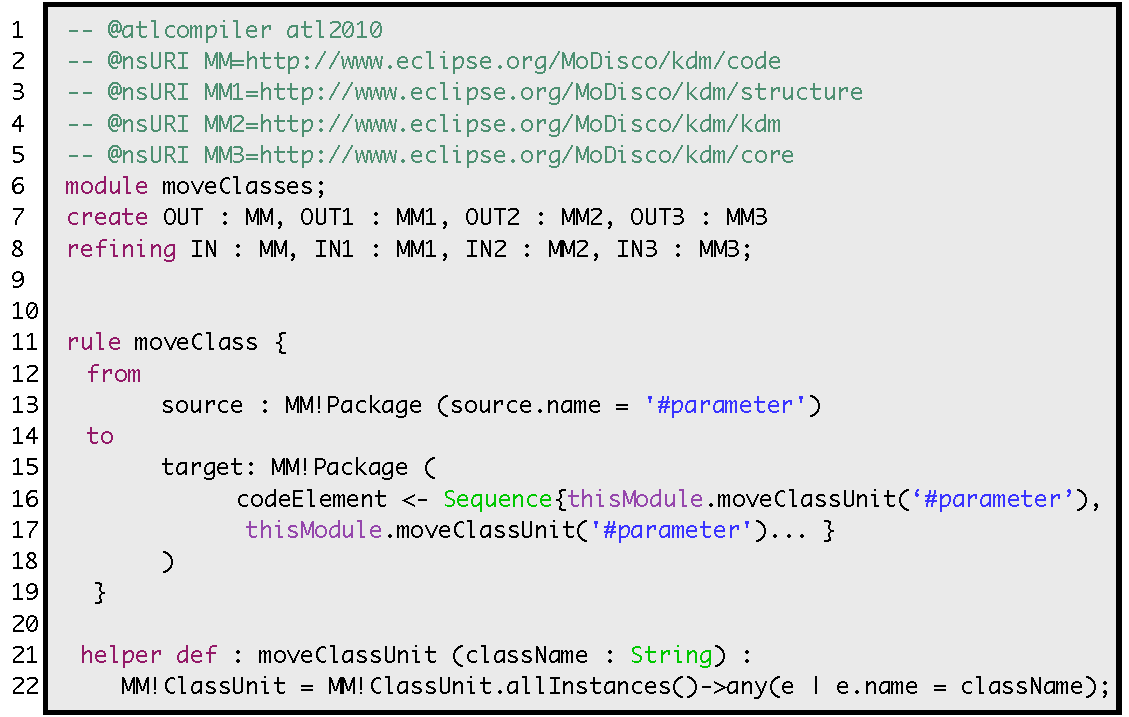
\includegraphics[scale=0.47]{figuras/ATLTRansformationLanguage}
	\caption{Chunk of code in ATL to perform the refactoring \textit{Move Class}.}
	\label{fig:ATLRefactoring}
\end{figure}


By inspecting this transformation/refactoring we can see important informations. For instance, lines 1 to 5 illustrate which KDM's level/packages are be affected by this transformation.  After, in line 6 it is possible to see the name of our transformation, \texttt{moveClasses}. Lines 7 and 8 represent the output and input models that conform to the KDM, e.g., the model used during the transformation/refactoring. 
%
With the \texttt{refining} mode (see Line 8 of Figure~\ref{fig:ATLRefactoring}), the ATL engine can focus on the ATL code dedicated to the generation of modified target elements. Other KDM elements (e.g. those that remain unchanged) are implicitly processed by the ATL engine.

%The keyword \texttt{refining} means informs to the ATL engine that  to the ATL engine that this transformation is \textit{in-place}

Line 11 a matched rule is defined. In fact, this rule represents the refactoring \textit{Move Class}. Occurrences of the input pattern may be filtered by introducing a \textit{guard}, a boolean condition that KDM model must satisfy (e.g., line 13). Lines 14 though 19 the refactoring \textit{Move Class} is actually defined. As can be seen, we are moving a set of \texttt{ClassUnit} by means of the helper (defined in lines 21 and 22). 
Almost all refactorings need some input parameters that should be properly instantiated by the user. For instance, consider the chuck of code written in ATL depicted in Figure~\ref{fig:ATLRefactoring}, lines 13, 16, and 17 (\texttt{\#parameter}). Therefore, before to apply the refactoring, the user should set the parameters. Considering our running example (depicted in Figure~\ref{fig:system}) the parameters would be: \texttt{Model}, \texttt{Student}, and \texttt{Instructor}, respectively. Afterward, this ATL is ready to be applied into a KDM instance.


%It is important to highlight that this chuck of code in written in ATL is not total functional - the engineer should set the parameters (\texttt{\#parameter}) 

%Refactorings are implemented by specifying its actions that have to be executed for applying the change. Most of them need also some input parameters that should be properly instantiated by the user. For instance, consider the chuck of code written in ATL depicted in Figure~\ref{fig:ATLRefactoring} 

\subsection{Propagate Changes} % (fold)
\label{sub:apply_refactoring}

In this step, all propagations regarding the refactoring \textit{Move Class} are implemented. In fact, this step is performed along with the step [B] using a set of rules defined in ATL. In Figure~\ref{fig:ATLPropagation} the ATL used to propagate the changes regarding the refactoring \textit{Move Class} is presented. As can be seen, there are three rules - each of them is used to propagated the change in a specific KDM package, respectively. The first rule is responsible to propagate the changes throughout the \texttt{Structure Package}, see lines 24 to 32. In line 26 the source pattern of the rules is defined by using OCL [17] guard stating the layers to be matched. After, is defined a target pattern (lines 29 -31) which is used to compute the \texttt{density} of an \texttt{AggregationRelationship} after the application of the refactoring \textit{Move Class}.

\begin{figure}[h]	
	\centering
	% Requires \usepackage{graphicx}
	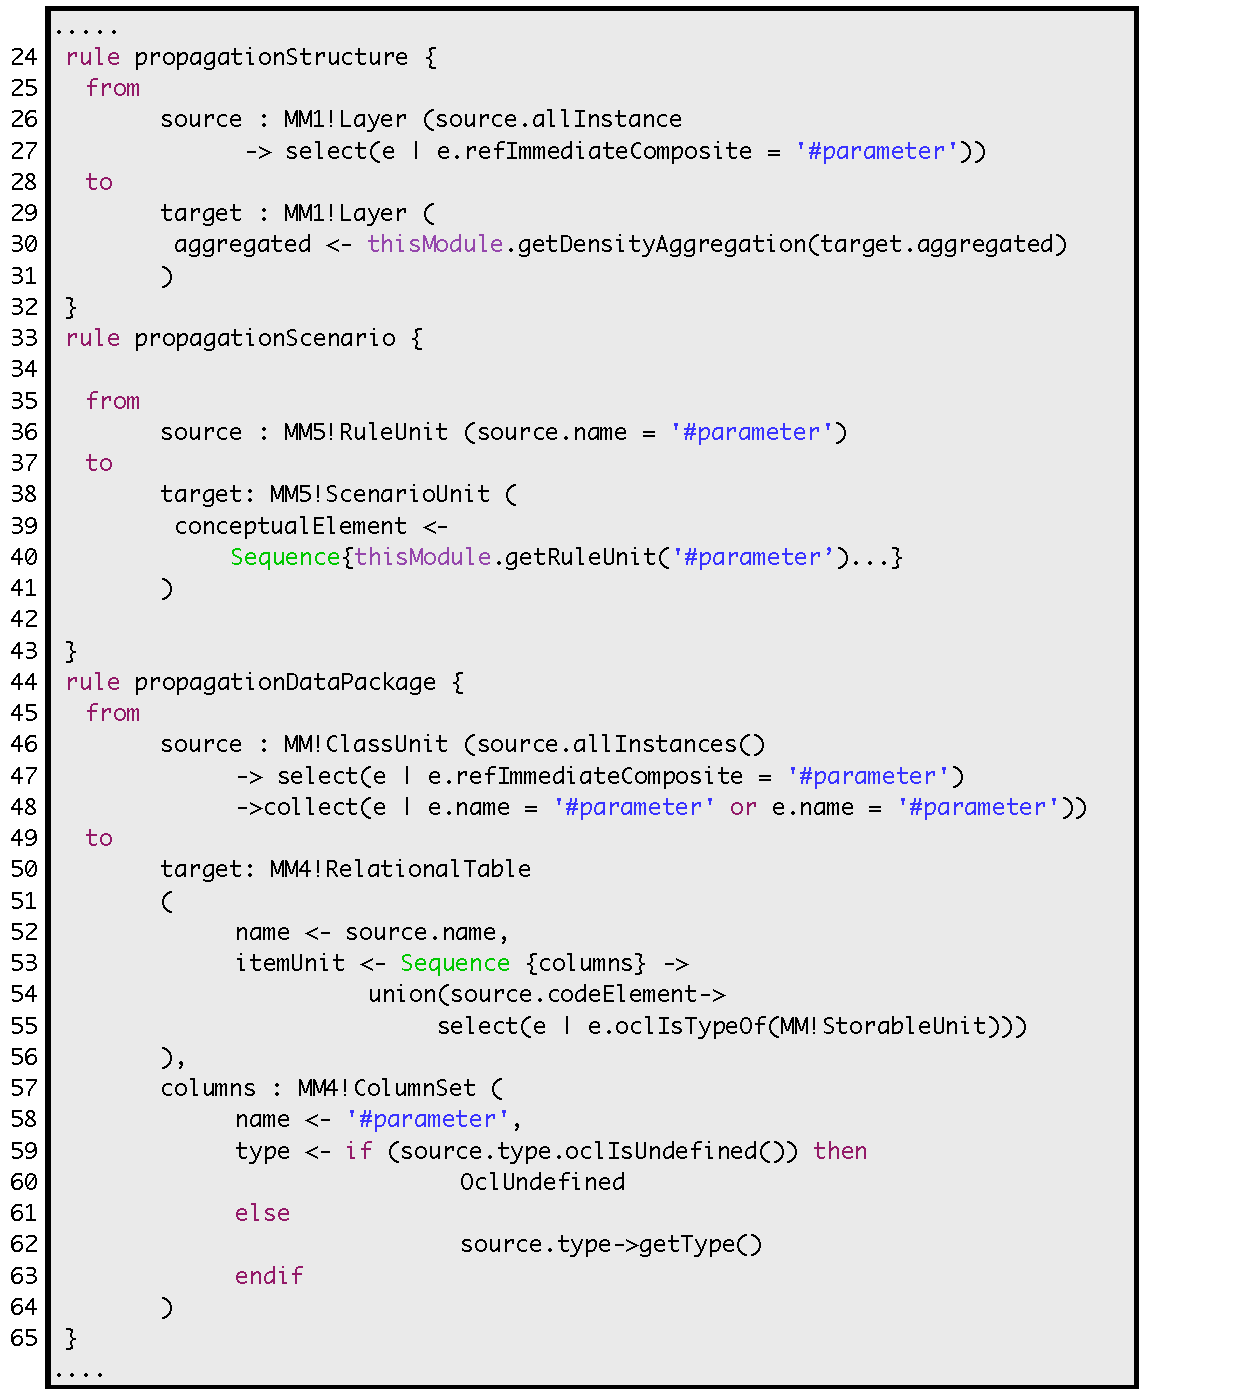
\includegraphics[scale=0.47]{figuras/propagationATLFormatted}
	\caption{Chunk of code in ATL to perform the propagation after the application of refactoring \textit{Move Class}.}
	\label{fig:ATLPropagation}
\end{figure}

The rule defined in lines 33 to 43 propagates the changes throughout the \texttt{Conceptual Package}. For instance,  the \texttt{RuleUnit 1.1} that is associated with \texttt{Instructor} should also be moved to corresponding scenario, i.e, the scenario that is associated with the package that contains now the class \texttt{Instructor} - \texttt{ScenarioUnit 3}. 

 Finally, the rule defined in lines 44 - 65 aims to propagate the change to the \texttt{Data Package}. For each moved \texttt{ClassUnit}, a \texttt{RelationalTable} instance has to be created. Their names have to correspond. The \texttt{itemUnit} %(a collection that contains \texttt{ColumnSet}) 
reference set has to contain all \texttt{ColumnSet} that have been created for each \texttt{StorableUnit} (metaclass that represent all the attributes that a class holds) as well as its types.

%In the step [C] all the changes, that where resulted by the refactoring  performed in step [b] need be propagate into all KDM's levels/package.  



